\section{LINEAR QUADRATIC REGULATOR DESIGN} \label{sec:control}

\subsection{Full-state feedback regulator} \label{sec:fullstate_design}

The bi-orthogonal basis generated by the Riesz-spectral operator $\mathfrak{A}$ in the LTI system $\mathbf{\Sigma(\mathfrak{A},\mathfrak{B},\mathfrak{C},-)}$ provides the foundation for solving the Operator Riccati Equation (ORE), a crucial step in the design of a Linear Quadratic Regulator (LQR). The objective is to \DIFdelbegin \DIFdel{derive a }\DIFdelend \DIFaddbegin \DIFadd{determine an offline }\DIFaddend feedback control law that \DIFdelbegin \DIFdel{minimizes the }\DIFdelend \DIFaddbegin \DIFadd{drives the system's states from an arbitrary initial condition to zero, thereby maintaining the system at its steady state. This is achieved within an optimal control framework, minimizing the }\DIFaddend infinite-time cost function \DIFdelbegin \DIFdel{, as }\DIFdelend defined in Equation~\ref{eq:cost_fun}\DIFdelbegin \DIFdel{, with }\DIFdelend \DIFaddbegin \DIFadd{. In this context, }\DIFaddend $\mathfrak{Q}$ and $\mathfrak{R}$ \DIFdelbegin \DIFdel{being positive semi-definite }\DIFdelend \DIFaddbegin \DIFadd{are self-adjoint coercive }\DIFaddend operators that penalize state deviations and control actions, respectively.

\begin{equation} \label{eq:cost_fun}
    J(\DIFdelbegin \DIFdel{x_0}\DIFdelend \DIFaddbegin \bm{x_0}\DIFaddend , u) = \int_{t=0}^{\infty} \langle \bm{x}(s), \mathfrak{Q} \bm{x}(s)\rangle + \langle u(s), \mathfrak{R} u(s)\rangle ds
\end{equation}

\subsubsection{Operator Riccati equation}

The LQR problem is solved by finding the unique positive semi-definite operator $\mathbf{\Pi}$, which satisfies the ORE presented in Equation~\ref{eq:ORE_1}. This operator is then used to compute the feedback gain that ensures optimal control of the system.

\begin{equation} \label{eq:ORE_1}
    \langle \mathfrak{A}^* \mathbf{\Pi} \bm{x}, \bm{y}\rangle + \langle \mathbf{\Pi} \mathfrak{A} \bm{x}, \bm{y} \rangle - \langle \mathbf{\Pi} \mathfrak{B} \mathfrak{R}^{-1} \mathfrak{B}^* \mathbf{\Pi} \bm{x}, \bm{y}\rangle + \langle \mathfrak{Q} \bm{x}, \bm{y}\rangle = 0
\end{equation}

Given that the solution to the ORE is unique for any set of functions in the domain of operator $\mathfrak{A}$, we can select $\bm{x} = \bm{\phi_m}$ and $\bm{y} = \bm{\phi_n}$, i.e. the eigenfunctions of $\mathfrak{A}$. Applying this choice, and noting that $\mathbf{\Pi}$ is self-adjoint, leads to the simplified Equation~\ref{eq:ORE_2}.

\begin{equation} \label{eq:ORE_2}
    \langle \mathbf{\Pi} \bm{\phi_m}, \mathfrak{A} \bm{\phi_n} \rangle
    + \langle \mathfrak{A} \bm{\phi_m}, \mathbf{\Pi} \bm{\phi_n} \rangle
    - \mathfrak{R}^{-1} \langle \mathfrak{B}^* \mathbf{\Pi} \bm{\phi_m}, \mathfrak{B}^* \mathbf{\Pi} \bm{\phi_n} \rangle 
    + \langle \mathfrak{Q} \bm{\phi_m}, \bm{\phi_n} \rangle = 0
\end{equation}

To ensure that the domain and range of $\mathbf{\Pi}$ match those of $\mathfrak{A}$ and $\mathfrak{A}^*$, respectively, $\mathbf{\Pi}$ can be expressed as an infinite series, as shown in Equation~\ref{eq:P}. The coefficients $p_{i,j}$ can be interpreted as elements of an infinite-dimensional matrix $\tilde{P}$, which represents the operator $\mathbf{\Pi}$. This forms the first step in converting the ORE to the corresponding Matrix Riccati Equation (MRE).

\begin{equation} \label{eq:P}
    \mathbf{\Pi} \DIFdelbegin \DIFdel{x }\DIFdelend \DIFaddbegin \bm{x} \DIFaddend \equiv \sum_{i=1}^{\infty}\sum_{j=1}^{\infty} p_{i,j} \langle \bm{x}, \bm{\psi_j} \rangle \bm{\psi_i} \qquad
    \forall {i,j}: \quad p_{i,j} \in \mathbb{C}
\end{equation}

\subsubsection{Obtaining $\mathfrak{B}$ and $\mathfrak{B}^*$}

Before further simplifying the ORE, it is essential to define the operators $\mathfrak{B}$ and $\mathfrak{B}^*$. Given the boundary-control nature of the system as seen in Equation~\ref{eq:BC}, $\mathfrak{B}$ is defined to properly project the control input $u \in \mathbb{R}^1$ onto the state space $X: L^2[0,1] \times L^2[0,1]$, as outlined in Equation~\ref{eq:B}.

\begin{equation} \label{eq:B}
    \mathfrak{B} u \equiv v(1-R)
    \begin{bmatrix}
        \delta(\zeta) \\ 0
    \end{bmatrix} \cdot u
\end{equation}

The adjoint operator $\mathfrak{B}^*$ is obtained by leveraging the properties of $\mathfrak{A}$ and $\mathfrak{A}^*$, i.e. their expressions as well as their domains (as shown in Equations~\ref{eq:operator_A}~and~\ref{eq:adjoint_A}), after applying integration by parts to the result of the inner products, as summarized in Equation~\ref{eq:B*}.

\begin{equation} \label{eq:B*}
    \begin{aligned}
        \langle \mathfrak{A} \bm{x} + \mathfrak{B} u, \bm{y} \rangle
        &= \langle \mathfrak{A} \bm{x}, \bm{y} \rangle
        + \langle \mathfrak{B} u, \bm{y} \rangle
        = \langle \bm{x}, \mathfrak{A}^* \bm{y}\rangle
        + \langle u, \mathfrak{B}^* \bm{y} \rangle \\
        \langle u, \mathfrak{B}^* \bm{y} \rangle
        &= \langle \mathfrak{A} \bm{x} + \mathfrak{B} u, \bm{y} \rangle
        - \langle \bm{x}, \mathfrak{A}^* \bm{y}\rangle
        \Rightarrow \hdots \\ \Rightarrow \mathfrak{B}^* (\cdot) &= \Bigl[ v(1-R) \int_0^1 \delta(\zeta) (\cdot) d\zeta \quad , \quad 0 \Bigr]
    \end{aligned}
\end{equation}

\subsubsection{Matrix Riccati equation}

Using the expression for $\mathbf{\Pi}$ in Equation~\ref{eq:P}, along with the derived $\mathfrak{B}^*$ from Equation~\ref{eq:B*}, and the eigenvalue problem $\mathfrak{A}\bm{\phi_i} = \lambda_i \bm{\phi_i}$, the ORE can be reformulated as the Matrix Riccati Equation (MRE) shown in Equation~\ref{eq:MRE}. Here, $\gamma_i \equiv v(1-R) \left. \psi_{1}^{(i)} \right|_{\zeta = 0}$, and $q_{m,n} = \langle \mathfrak{Q} \bm{\phi_m}, \bm{\phi_n} \rangle$.

\begin{equation}\label{eq:MRE}
    p_{n,m} (\lambda_m + \overline{\lambda_n})
    - \mathfrak{R}^{-1} \langle \sum_{i=1}^\infty p_{i,m} \gamma_i, \sum_{i=1}^\infty p_{i,n} \gamma_i \rangle
    + q_{m,n} = 0
\end{equation}

Due to the infinite-dimensional nature of $\tilde{P}$, a numerical solution is impractical. This challenge is addressed by selecting the first $N$ eigenmodes of the system as its dominant modes. This means truncating the infinite sums in the MRE and reducing the infinite-dimensional system to a finite set of nonlinear algebraic equations that can be solved to obtain an equivalent $N \times N$ matrix $P$, i.e. a truncated approximation of matrix $\tilde{P}$. The optimal full-state feedback gain is then calculated using Equation~\ref{eq:fullstate_gain}, ensuring closed-loop stability.

\begin{equation} \label{eq:fullstate_gain}
    \begin{aligned}
        u(t) &= - \langle \bm{K}(\zeta), \bm{x}(\zeta, t) \rangle = - \mathfrak{B}^* \mathbf{\Pi} \bm{x}(\zeta, t) \\
        &= - \sum_{i=1}^N\sum_{j=1}^N p_{i,j} \langle \bm{x}(\zeta, t), \bm{\psi_j}(\zeta) \rangle \gamma_i \\
        &= - \sum_{i=1}^N\sum_{j=1}^N p_{i,j} \gamma_i \int_0^1 \bm{x}(\zeta, t) \cdot \overline{\bm{\psi_j}}(\zeta) d\zeta \\
        &= - \int_0^1 \sum_{i=1}^N\sum_{j=1}^N p_{i,j} \gamma_i \overline{\bm{\psi_j}}(\zeta) \cdot \bm{x}(\zeta, t) d\zeta \\
        \Rightarrow \bm{K}(\zeta) &\equiv \sum_{i=1}^N\sum_{j=1}^N p_{i,j} \gamma_i \overline{\bm{\psi_j}}(\zeta)
    \end{aligned}
\end{equation}

The computed gain is a function of space and is calculated offline. The control action at any given time instance is the inner product of this gain with the current state of the system, thus justifying the term ``full-state'' feedback. The dynamics of the resulting closed-loop full-state feedback system may be described by the state-space representation shown in Equation~\ref{eq:fullstate_ss}.

\begin{equation}
    \begin{aligned} \label{eq:fullstate_ss}
        \dot{x}(\zeta, t) &= \mathfrak{A} \bm{x}(\zeta, t) + \mathfrak{B} u(t) \\
        &= (\mathfrak{A} - \mathfrak{B} \bm{K}) \, \bm{x}(\zeta, t) \\
        &= \mathfrak{A}_{reg} \, \bm{x}(\zeta, t)
    \end{aligned}
\end{equation}

By selecting $\mathfrak{Q} = 0.05$ as a constant function over $\zeta = [0,1]$, and $\mathfrak{R} = 50$, the full-state feedback gain is obtained and represented in Figure~\ref{fig:k_modes}. The obtained gains are used to design the optimal full-state feedback regulator to stabilize the control system. A block diagram representation of the full-state feedback control system is shown in Figure~\ref{fig:block_diagram}.

\begin{figure}[!htbp]
    \centering
    \begin{subfigure}[b]{0.45\textwidth}
        \centering
        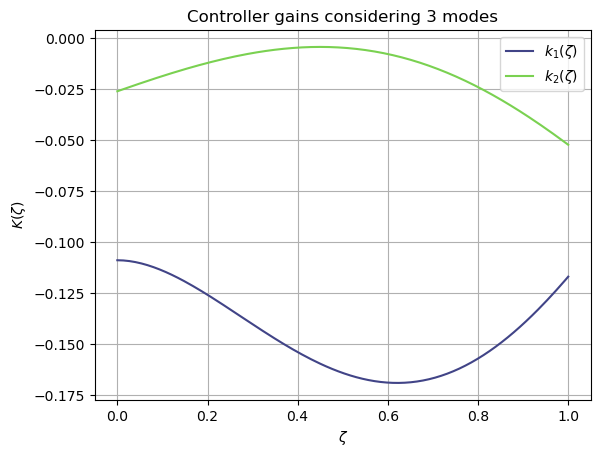
\includegraphics[width=\textwidth]{Figures/k_3.png}
        \caption{$N = 3$}
        \label{fig:k_3}
    \end{subfigure}
    \hfill
    \begin{subfigure}[b]{0.45\textwidth}
        \centering
        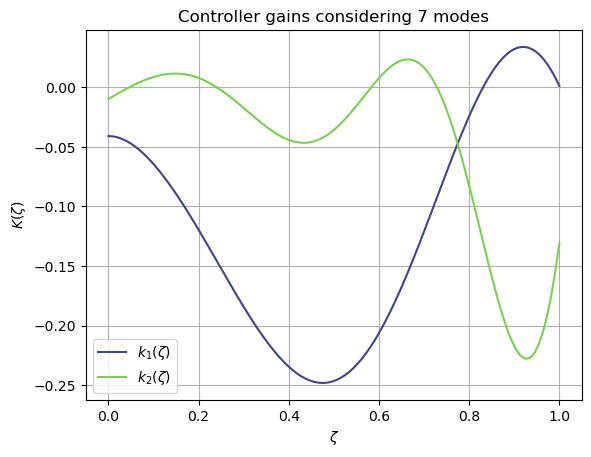
\includegraphics[width=\textwidth]{Figures/k_7.png}
        \caption{$N = 7$}
        \label{fig:k_7}
    \end{subfigure}
    \caption{Full-state feedback gain $\bm{K}(\zeta)$ utilizing the first $N$ modes of the system given by Equation~(\ref{eq:fullstate_gain}).}
    \label{fig:k_modes}
\end{figure}

\begin{figure}[!htbp]
    \centering
    \begin{tikzpicture}[node distance=2cm]
        \node (plant) [block_1] {Plant};
        \node (regulator) [block_1, below of=plant] {Regulator};
        \draw [arrow] (plant.south) -- node[midway, right] {$\bm{x}(\zeta,t)$} (regulator.north);
        \draw [arrow] (regulator.west) -- ++(-1,0) |- node[near end, above] {$u(t)$} (plant.west);
        \draw [arrow] (plant.east) -- node[midway, above] {$y(t)$} ++(1,0);
    \end{tikzpicture}
    \caption{Block diagram representation of the optimal full-state feedback control system.}
    \label{fig:block_diagram}
\end{figure}

\subsection{Output feedback compensator} \label{sec:output_design}

Thus far, the optimal regulator is designed under the assumption that it has full access to the system's states. However, this assumption is not feasible in realistic applications. To address this, an observer is introduced to estimate and reconstruct the states by measuring the system's output in real time, and providing the regulator with the reconstructed states to further stabilize the system. The output, in this context, is taken as the concentration at the reactor outlet, as defined in Equation~\ref{eq:BC}. This leads to the definition of the output operator $\mathfrak{C}$ in the linear time-invariant (LTI) system $\mathbf{\Sigma(\mathfrak{A},\mathfrak{B},\mathfrak{C},-)}$, which is subsequently used to determine the observer gain, $\bm{L}(\zeta)$. The formulation is shown in Equation~\ref{eq:C}:

\begin{equation} \label{eq:C}
    \mathfrak{C} \equiv \begin{bmatrix}
        \int_0^1 \delta(\zeta-1) ( \cdot ) d\zeta \quad , \quad 0
    \end{bmatrix}
\end{equation}

where $\delta(\zeta)$ denotes the Dirac delta function. Regarding the choice of observer, Luenberger-based observers are well-suited for infinite-dimensional systems when the system parameters are perfectly known \autocite{ali2015reviewobserver}. Among the various methods to compute the gain for this class of observers, pole-placement is a solid, straightforward, and reliable approach for state reconstruction. To ensure that the state reconstruction dynamics converge more quickly than the regulation dynamics, the poles of the observer-based controller are placed to the left of the poles of the full-state feedback controller. This practice is common in the design of observer-based controllers for infinite-dimensional systems \autocite{morrisbook}. The observer gain in Figure~\ref{fig:L_modes} is obtained by limiting the eigenmodes of the observer-based controller to have real parts that are at least 3 times more negative than the real part of the dominant eigenmodes of the full-state feedback system. This is done for the case where the first 7 modes of the system are considered for designing the controller. The first few eigenvalues of the observer-based controller and the full-state feedback controller, along with the eigenvalues of the open-loop system are shown in Figure~\ref{fig:eigs} to demonstrate the pole placement strategy explained above. It can be confirmed that both control systems have eigenvalues with negative real parts, ensuring stability. Note that the eigenvalues of both control systems are identical after the 7th mode, as the real parts of these eigenvalues are already sufficiently negative.

\begin{figure}[!htbp]
    \centering
    \includesvg[inkscapelatex=false, width=0.5\textwidth, keepaspectratio]{Figures/L.svg}
    \caption{Observer gain $\bm{L}(\zeta)$.}
    \label{fig:L_modes}
\end{figure}

\begin{figure}[!htbp]
    \centering
    \includesvg[inkscapelatex=false, width=0.5\textwidth, keepaspectratio]{Figures/pole_placement.svg}
    \caption{Eigenvalues of the observer-based controller, full-state feedback controller, and open-loop system.}
    \label{fig:eigs}
\end{figure}

The dynamics of the augmented observer-controller system are described by the state-space representation shown in Equation~\ref{eq:observer_ss}, where $\hat{\bm{x}}(\zeta, t)$ and $\bm{e}(\zeta, t)$ refer to the estimated state and the state estimation error, respectively. A block diagram representation of the output feedback control system is also shown in Figure~\ref{fig:block_diagram_observer}.

\begin{figure}[!htbp]
    \centering
    \begin{tikzpicture}[node distance=2cm]
        \node (plant) [block_2, minimum width=4cm] {Plant};
        \node (regulator) [block_2, below of=plant, xshift=-1cm, yshift=-1cm] {Optimal Gain};
        \node (observer) [block_2, below of=plant, xshift=1cm, yshift=0.5cm] {Observer};
        \draw [arrow] (plant.east) -- node[midway, above] {$y(t)$} ++(2,0);
        \draw [arrow] (plant.east) ++(1,0) |- (observer.east);
        \draw [arrow] (observer.south) -- ++(0,-1) node[midway, right] {$\hat{\bm{x}}(\zeta,t)$} -- (regulator.east);    
        \draw [arrow] (regulator.west) -- ++(-1,0) |- (plant.west);
        \draw [arrow] (regulator.west) ++(-1,1.5) coordinate(start) -- node[near start, left, xshift=-0.75cm] {$u(t)$} (observer.west);
    \end{tikzpicture}
    \caption{Block diagram representation of the observer-based output feedback control system.}
    \label{fig:block_diagram_observer}
\end{figure}

\begin{equation}
    \begin{aligned} \label{eq:observer_ss}
        \left[\begin{array}{c}
            \dot{\bm{x}}(\zeta,t) \\ \hline \dot{\hat{\bm{x}}}(\zeta,t)
        \end{array}\right] &= 
        \left[
            \begin{array}{c|c}
                \mathfrak{A} & -\mathfrak{B} \bm{K} \\ \hline
                \bm{L} \mathfrak{C} & \mathfrak{A} - \mathfrak{B} \bm{K} - \bm{L} \mathfrak{C}
            \end{array}
        \right]
        \left[ \begin{array}{c}
            \bm{x}(\zeta,t) \\ \hline \hat{\bm{x}}(\zeta,t) \end{array}
            \right] \\
        \dot{\bm{e}}(\zeta,t) &= \left[ \dot{\bm{x}}(\zeta,t) - \dot{\hat{\bm{x}}}(\zeta,t) \right] \\
        &= (\mathfrak{A} - \bm{L} \mathfrak{C}) \, \bm{e}(\zeta,t) \\
        &= \mathfrak{A}_{est} \, \bm{e}(\zeta,t)
    \end{aligned}
\end{equation}
